\documentclass[
% -- opções da classe memoir --
12pt,				% tamanho da fonte
%openright,			% capítulos começam em pág ímpar (insere página vazia caso preciso)
%openany,
twoside,			% para impressão em verso e anverso. Oposto a oneside
a4paper,			% tamanho do papel.
% -- opções da classe abntex2 --
%chapter=TITLE,		% títulos de capítulos convertidos em letras maiúsculas
%section=TITLE,		% títulos de seções convertidos em letras maiúsculas
%subsection=TITLE,	% títulos de subseções convertidos em letras maiúsculas
%subsubsection=TITLE,% títulos de subsubseções convertidos em letras maiúsculas
% -- opções do pacote babel --
english,			% idioma adicional para hifenização
brazil,				% o último idioma é o principal do documento
]{abntex2}

\usepackage[alf]{abntex2cite}	% Citações padrão ABNT

\usepackage{cmap}				% Mapear caracteres especiais no PDF
\usepackage{lmodern}			% Usa a fonte Latin Modern

\usepackage{amsmath}
\usepackage{amsfonts}
\usepackage{amssymb}
\usepackage{algpseudocode}
\usepackage{algorithm}

\usepackage{graphicx}			% Inclusão de gráficos

\usepackage[T1]{fontenc}		% Selecao de codigos de fonte.
\usepackage[utf8]{inputenc}		% Codificacao do documento (conversão automática dos acentos)

\addto\captionsbrazil{%
\def\bibname{References}%
}

\addto\captionsbrazil{
  \renewcommand{\contentsname}%
    {Contents}%
}

\titulo{A Hybrid Heuristic for the Multi-objective Knapsack Problem}
\autor{Marcos Daniel V. Baroni}
\local{Vitória - Espírito Santo - Brasil}
\data{November 27, 2017}
\orientador[Advisor:]{Dr. Flávio Miguel Varejão}
%\coorientador{Equipe \abnTeX}
\instituicao{%
  Universidade Feredal do Espírito Santo -- UFES
  \par
  Departamento de Informática
  \par
  Programa de Pós-Graduação em Informática}
\tipotrabalho{Tese (Doutorado)}
% O preambulo deve conter o tipo do trabalho, o objetivo,
% o nome da instituição e a área de concentração
\preambulo{Tese de Doutorado apresentada de acordo
com o regimento do Programa de Pós-graduação
em Informática da Universidade
Federal do Espírito Santo.}

\makeindex

\begin{document}

%%%%%%%%%%%%%%%%%%%%%%%%
% Folhas               %
%%%%%%%%%%%%%%%%%%%%%%%%
\imprimircapa
\imprimirfolhaderosto*

\newcommand{\dtree}[1]{$#1$-d~tree}
\newcommand{\kdtree}{\dtree{k}}
\newcommand{\bsym}[1]{\boldsymbol{#1}}
%\newcommand{\sol}[1]{\boldsymbol{#1}}
\newcommand{\sol}[1]{#1}
\newcommand{\pnt}[1]{pnt(\sol{#1})}
\newcommand{\fsol}[1]{f(\sol{#1})}
\newcommand{\np}{m}
\newcommand{\nphard}{$\mathcal{NP}$-Hard}
\newcommand{\missingI}[1]{}
\newcommand{\missing}[1]{
  \begin{framed}
    {\scriptsize  #1}
  \end{framed}
}
\newcommand{\weight}[1]{w(\sol{#1})}
\newcommand{\obj}[2]{f_{#1}(\sol{#2})}
\newcommand{\bigweight}[1]{w\big(\sol{#1}\big)}
\newcommand{\dom}[2]{dom(\sol{#1}, \sol{#2})}
\newcommand{\domk}[2]{dom_k(\sol{#1}, \sol{#2})}
\newcommand{\setIN}{\{1, \ldots, n\}}
\newcommand{\ext}[2]{ext(\sol{#1}, \sol{#2})}
\newcommand{\domLess}[2]{ \sol{#1} \prec \sol{#2} }
%\newcommand{\logicAnd}{ \textrm{ and } }
\newcommand{\logicAnd}{ \land }
\newcommand{\logicOr}{ \lor}
\newcommand{\solSetA}{ Q }
\newcommand{\solSetB}{ R }
\newcommand{\solSett}{ S_* }
\newcommand{\solSet}{ S }
\newcommand{\rord}{\mathcal{O}_{rev}}
\newcommand{\cb}[2]{cb^{#1}(#2)}  % cost-benefit function
\renewcommand{\leq}{\leqslant}
\renewcommand{\geq}{\geqslant}
\newcommand{\floor}[1]{\left \lfloor{#1}\right \rfloor}

% bar graphs configs
\newcommand{\cmpH}{4.0cm}
\newcommand{\cmpW}{7cm}
\newcommand{\legX}{0.45}
\newcommand{\legY}{-0.30}
\newcommand{\scecore}{SCEcr }
\newcommand{\mokp}{MOKP}
\newcommand{\paretoset}{conjunto Pareto}
\newcommand{\paretosetII}{conjunto Pareto-ótimo}
\newcommand{\knapsackdominates}{domina segundo a mochila}

% big bullet
\newcommand{\bbt}{\,\begin{picture}(-1,1)(-1,-2)\circle*{5}\end{picture}\ }

\begin{folhadeaprovacao}

  \begin{center}
    {\ABNTEXchapterfont\large\imprimirautor}

    \vspace*{\fill}\vspace*{\fill}
    {\ABNTEXchapterfont\bfseries\Large\imprimirtitulo}
    \vspace*{\fill}
    
    \hspace{.45\textwidth}
    \begin{minipage}{.5\textwidth}
        \imprimirpreambulo
    \end{minipage}%
    \vspace*{\fill}
   \end{center}
    
   Work approved. \imprimirlocal, November 27, 2017:

   \assinatura{\textbf{\imprimirorientador} \\ Advisor} 
   \assinatura{\textbf{Dr.ª Simone de Lima Martins} \\ Guest}
   \assinatura{\textbf{Dr. Arlindo Gomes de Alvarenga} \\ Guest}
   %\assinatura{\textbf{Professor} \\ Convidado 3}
   %\assinatura{\textbf{Professor} \\ Convidado 4}
      
   \begin{center}
    \vspace*{0.5cm}
    {\large\imprimirlocal}
    \par
    {\large\imprimirdata}
    \vspace*{1cm}
  \end{center}
  
\end{folhadeaprovacao}


\begin{resumo}
Diversos problemas reais envolvem a otimização simultânea de múltiplos critérios,
os quais são, geralmente, conflitantes entre si.
Estes problemas são denominados multiobjetivo e
não possuem uma única solução, mas um conjunto de soluções de interesse, denominadas soluções
eficientes ou não dominadas.
Um dos grande desafios a serem enfrentados na resolução deste tipo de problema é o
tamanho do conjunto solução, que tende a crescer rapidamente dado o tamanho da instância,
degradando a performance dos algoritmos.
Dentre os problemas multiobjetivos mais estudados está o problema da mochila multiobjetivo,
pelo qual diversos problemas reais podem ser modelados.
Este trabalho propõe a aceleração do processo de solução do problema da mochila multiobjetivo,
através da utilizando da \kdtree{} como estrutura de indexação multidimensional
para auxiliar a manipulação das soluções.
A performance da abordagem é analisada através de experimentos
computacionais, realizados no contexto exato utilizando um algoritmo estado da arte.
Testes também são realizados no contexto heurístico, utilizando a adaptação
de uma meta-heurística para o problema em questão, sendo esta também uma contribuição do presente trabalho.
Segundo os resultados, para o contexto exato a proposta foi eficaz, apresentam speedup de até $2.3$
para casos bi-objetivo e $15.5$ em casos 3-objetivo, não sendo porém
eficaz no contexto heurístico, apresentando pouco impacto no tempo computacional.
Em todos os casos, porém, houve considerável redução no número de avaliações de soluções.

\vspace{\onelineskip}

\noindent
\textbf{Palavras Chave}:
Problema da Mochila Multiobjetivo,
Indexação Multidimensional,
Meta-heurística,
Algoritmo Exato.
\end{resumo}


\begin{resumo}[Abstract]
\begin{otherlanguage*}{english}
Several real problems involve the simultaneous optimization of multiple criteria,
which are generally conflicting with each other.
These problems are called multiobjective and
do not have a single solution, but a set of solutions of interest, called efficient solutions
or non-dominated solutions.
One of the great challenges to be faced in solving this type of problem is the
size of the solution set, which tends to grow rapidly given the size of the instance,
degrading algorithms performance.
Among the most studied multiobjective problems is the multiobjective knapsack problem,
by which several real problems can be modeled.
This work proposes the acceleration of the resolution process of the multiobjective knapsack problem,
through the use of a \kdtree {} as a multidimensional index structure
to assist the manipulation of solutions.
The performance of the approach is analyzed through computational experiments,
performed in the exact context using a state-of-the-art algorithm.
Tests are also performed in the heuristic context, using the adaptation
of a meta-heuristic for the problem in question, being also a contribution of the present work.
According to the results, the proposal was effective for the exact context, presenting a speedup up to $2.3$
for bi-objective cases and $15.5$ for 3-objective cases, but not
effective in the heuristic context, presenting little impact on computational time.
In all cases, however, there was a considerable reduction in the number of solutions evaluations.
\vspace{\onelineskip}

\noindent

\textbf{Keywords}:
Multiobjective Knapsack Problem,
Multidimensional Indexing,
Metaheuristic,
Exact Algorithm.
\end{otherlanguage*}
\end{resumo}

% Falar brevemente sobre o MOKP
% Falar brevemente sore a estratégia de indexação
% Resumir os resultados obtidos

%\missingt{
%Observar as 5 regras:\\
%1. A general statement introducing the broad research area of the particular topic being investigated;\\
%2. An explanation of the specific problem (difficulty, obstacle, challenge) to be solved;\\
%3. A review of existing or standard solutions to this problem and their limitations;\\
%4. An outline of the proposed new solution;\\
%5. A summary of how the solution was evaluated and what the outcomes of the evaluation were.
%}

% 1. Uma declaração geral introduzindo a área de pesquisa;
% 2. Uma explicação espeficica do problema
% 3.
%
%

%%%%%%%%%%%%%%%%%%%%%%%%
%  Sumário             %
%%%%%%%%%%%%%%%%%%%%%%%%
\pdfbookmark[0]{\contentsname}{toc}
\tableofcontents*

%%%%%%%%%%%%%%%%%%%%%%%%
%  Texto               %
%%%%%%%%%%%%%%%%%%%%%%%%
% Introdução
\chapter{Introdução}
%  - The problem and its application
%  - Literature background
%  - The Bazgan algorithm
%  - Our approach (motivation and use of KDTRee)
%  - Article structure


% Multi-objective Knapsack Problem
\chapter{O Problema da Mochila Multi-objetivo}
% Breve definicao de multiobjective opt
A general multiobjective optimization problem can be described as a vector
function $f$ that maps a tuple of $n$ parameters (decision variables) to a tuple
of $\np$ objectives.
Formally:
\begin{align*}
  \text{min/max} ~ \sol{y} &= f(\sol{x}) = 
    \big(f_1(\sol{x})
    ,f_2(\sol{x})
    ,\ldots
    ,f_{\np}(\sol{x})\big) \\
  \text{subject to} ~ \sol{x} & = (x_1, x_2, \ldots, x_n) \in X
\end{align*}
where $\sol{x}$ is called the \emph{decision vector} or \emph{solution}, $X$ denotes the set
of feasible solutions, and $\sol{y}$ is the \emph{objective vector} or \emph{criterion vector} where
each objective has to be minimized (or maximized).

Considering two decision vectors $\sol{a}, \sol{b} \in X$, $a$ is said to
\emph{dominate} $b$ if, and only if:
\begin{align*}
    \forall i &\in \{1, 2, \ldots, \np\}: f_i(\sol{a}) \geq f_i(\sol{b}) \\
    \exists j &\in \{1, 2, \ldots, \np\}: f_j(\sol{a}) > f_j(\sol{b})
\end{align*}

A solution $\sol{a} \in X$ is called \emph{efficient} or \emph{non-dominated}
if there is not other feasible solution $\sol{b} \in X$ such that $\sol{b}$ dominates $\sol{a}$.
The set of solutions of a multiobjective optimization problem consists of all efficient solutions.
This set is known as \emph{Pareto optimal}.

The instance of a multiobjective knapsack problem with $\np$
objectives consists of an integer capacity $W > 0$ and $n$ items.
Each item $i$ has a positive weight $w^i$ and $\np$ non negative integer
profits $p_{i}^{1}, \ldots, p_{i}^{\np}$.
A solution is represented by a vector $\sol{x} = (x_1, \ldots, x_n)$ of binary
decision variables $x_i$, such that $x_i = 1$ if item $i$ is included in the
solution and $0$ otherwise, satisfing the capacity of the knapsack.
For any instance of the problem, we aim at determining the set of efficient solutions.

Formally the definition of the problem is:
\begin{align*}
    \text{max   } & f(\sol{x}) = 
      \big(f_1(\sol{x}) ,f_2(\sol{x}) ,\ldots ,f_{\np}(\sol{x})\big) \\
    \text{subject to   } & w(\sol{x}) < W \\
    & x_{i} \in \{0, 1\} \quad i = 1, \ldots, n \\
    \text{where} \phantom{mmmmm} \\
    f_j(\sol{x}) &= \sum_{i=1}^{n} v^j_i x_i \quad j = 1, \ldots, \np \\
    w(\sol{x}) &= \sum_{i=1}^{n} w_i x_i
\end{align*}

The MOKP is considered a \nphard{} problem, since it is a generalization
of the well-known 0$-$1 knapsack problem and
it is quite difficult to determine the Pareto optimal set for the MOKP,
especially for high dimension instances, in which the Pareto set it self tends
to grow exponentially.
For this reason, the development of methods efficiently deal with high-dimension
instances is...

% Definições, Propriedados e teoremas para o MOKP: dominancia


\section{O Problema da Mochila Multi-objetivo Uni-dimensional}
O algoritmo de Nemhauser e Ullmann é um algorimto de programação dinâmica
que resolve problemas da mochila de forma genérica aplicando o conceito de
dominância da mochila para remover soluções parciais que não resultarão em
soluções eficientes, ou seja, soluções que irão compor o \paretoset (conjunto solução).

\begin{algorithm}
  \caption{O algoritmo de Nemhauser e Ullmann para o \mokp.}
  \label{alg:nemull}
  \Kw{$\bsym{p}, \bsym{w}, W$}
\Begin{
  \SetAlgoLined
  $S_0 = \{(0, \ldots, 0)\}$\;
  \For{$k \gets 1, n$}{
    $S_k \gets S_{k-1} \cup \big\{(s^1 + p_k^1, \ldots, s^\np + p_k^\np, s^{\np+1} + w_k)\;$\
    $\phantom{S_k \gets S_{k-1} \cup \;} \big| \; s^{\np+1} + w_k \leq W, \: s \in S_{k-1} \big\}$\;
  }
  $P = \{ s \in S_n \:|\: \nexists (a \in S_n \;|\; a \dom s)\}$\;
  \textbf{return} $P$\;
}

\end{algorithm}

O algoritmo inicia definindo uma solução inicial $S^0$ contendo apenas a solução
vazia (linha 2).
Na $k$-ésimo iteração o algoritmo recebe um conjunto $S^{k-1}$ contendo
soluções exclusivamente compostas pelos primeiros ${k-1}$ itens,
ou seja, $\forall\sol{x} \in S^{k-1}, \sol{x} \subseteq \{1, \ldots, k-1\}$.
O conjunto $S^{k-1}$ é então expandido adicionando-se uma cópia de cada uma
das suas soluções mas desta vez incluindo o $k$-ésimo item (linha 4),
formando o conjunto $S^k_*$, o qual possui o dobro da cardinalidade de $S^{k-1}$.
O conjunto $S^k_*$..

Apesar de sua simplicidade o Algoritmo~\ref{alg:nemull} é consideravelmente poderoso.
Contudo o potencial crescimento exponencial do \paretoset para o \mokp
compromete severamente o seu desempenho.
Uma forma de atacar este problema é tentar reduzir ainda mais a quantidade de
soluções parciais manuseadas durante as iterações do algoritmo.
Três propostas...


% KD-tree
\chapter{A k-d tree}
% Falar sobre a utilização de estrutura de dados.

\section{Verificação de dominância e a busca de faixa}

Como dito anteriormente, solucionar um problema multi-objetivo significa
apresentar o seu \paretoset{}, ou seja, o conjunto de soluções não dominadas.
Geralmente o processo de solução compreende-se em contruir este conjunto de
soluções de forma incremental.
Por este motivo, um dos procedimentos mais executados durante o processo é
verificar se uma determinada solução é dominada por alguma outra solução
existente num conjunto candidato.
Um algoritmo pode até mesmo necessitar de extrair um cojunto cobertura, ou seja,
extrair todas as soluções não-dominadas de um grande conjuto de soluções.

Esta operação deve demandar exforço quadrático sobre o número total de soluções
se implementada como uma comparação par-a-par.
Entretanto, se as soluções forem interpretadas como pontos em um espaço
multi-dimensional, podemos deduzir da Equação~\ref{eq:dom} que esta operação
corresponde em verificar a existência um ponto numa determinada região
do espaço. O mesmo pode ser considerado no caso mais específico para a dominância
da mochila, segundo a Equação~???.
Formalmente:
\begin{align*}
    & x \dom y \; \Longleftrightarrow \; \pnt{y} \in R(\sol{x}) \\
  \text{where} \phantom{mmmmm} \\
    \pnt{x} &= \big(\obj{1}{x}, \ldots, \obj{\np}{x}, \weight{x}\big) \\
    R(\sol{x}) &= \left\{ a \in \mathbb{R}^{\np+1} \;\middle|\;
      a_{\np+1} \leq \weight{x}
      \, \text{ and } \,
      a_i \geq \obj{i}{x}, \; i \in \{1, \ldots, \np\}
      \right\}
\end{align*}

\missing{Colocar referência para a equação de dominância da mochila (texto acima).}

O problema de determinar a existência de um ponto numa determinada região do
espaço é já bem conhecido da computação e chama-se problema da
\emph{busca de baixa} (ou \emph{range search} em ingês)~\cite{agarwal1999geometric}.
O problema de busca de faixa é largamente aplicado, por exemplo, na área da
computação gráfica e jogos, onde é necessário se verificar a colisão entre pontos e polígonos.
Para se ter uma solução eficiente deste problema evitando o esforço computacional
quadrático, os pontos devem ser indexados multidimensional.....
\missing{Melhorar parágrafo acima e conferir texto inicial do parágrafo abaixo.}

Devido a sua simplicidade e eficiência, a estrutura de dados mais utilizada
para o problema é a \emph{\kdtree}~\cite{preparata2012computational}.
Proposta por Jon Louis Bentley em 1957~\cite{bentley1975}, a \kdtree{} é um tipo de
árvore binária de construção simples e baixa utilização de memória.
Apesar de sua simplicidade, além da operação de buca de faixa, a \kdtree{}
suporta outras operações como busca de vizinho mais próximo.
Por este motivo é também bastante utilizada em algoritmos de
clasterização~\cite{kanungo2002efficient, indyk1998approximate}
e renderização gráfica~\cite{owens2007survey}.

Como uma árvore binária comum, a cada nível recursivo da árvore
a \kdtree{} subdivide os dados em duas partes.
Porém, diferentemente de uma árvore de busca binária comum, as quais utilizam
apenas uma \emph{chave} em todos os níveis da árvore, a \kdtree{} utiliza um
total de $k$ chaves fazendo um revezamento circular entre as chaves à medida
que caminha nos níveis da árvore.

A Figura~\ref{fig:kdom-kd} apresenta (a) um conjunto de pontos dispostos num
espaço bi-dimensional e indexados por uma (b) \dtree{2}.
O primeiro e terceiro nível da \dtree{2} indexa a componente $x$ dos pontos,
enquanto o segundo nível indexa a componente $y$.
Cada ponto indexado pela árvore subdivide o espaço em dois de acordo
com o valor da componente que está sendo indexada.
A subdivisão do espaço é representada na figura por uma linha mais grossa.

\begin{figure}[H]
  \centering
  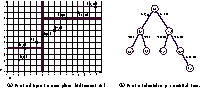
\includegraphics[scale=4.8]{img/kdt/dom-kd}
  \caption{Exemplo de pontos indexados por uma \kdtree{}.}
  \label{fig:kdom-kd}
\end{figure}

A Figura~\ref{fig:query} apresenta um exemplo de operação de verificação de
dominância utilizando uma \dtree{2} como estrutura de indexação.
A área acinzentada não tem intersecção com a área dominada pelo ponto $x$
(área hachurada), portanto as soluções dentro da área acinzentada não são
avaliadas.

\missing{Propor passo-a-passo da operação.}

\begin{figure}[H]
  \centering
  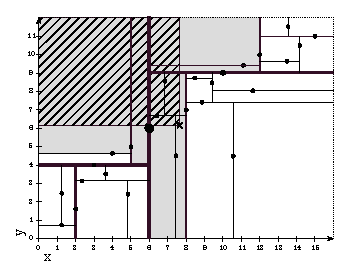
\includegraphics[scale=1.7]{img/kdt/query}
  \caption{Exemplo de operação de verificação de dominância utilizando a \kdtree{}.}
  \label{fig:query}
\end{figure}

Com relação à eficiência da \kdtree{} é importante considerar que não é
recomendável escalar de forma arbitrária o número $k$ de dimensões
indexadas pela \kdtree{}, esperando assim escalar também sua eficiência.
Mesmo que o dado possua todas estas dimensões.
Como regra geral considera-se que um \kdtree{} é adequada para indexar um
conjunto com $n$ pontos se $n$ não for muito maior que $2^k$\cite{toth2004handbook},
caso contrário, a performance da \kdtree{} se assemelhará a de uma busca
linear exaustiva.

Espera-se que a \kdtree{} auxilie as operações de verificação de dominância
\emph{podando} uma grande quantidade de soluções, demandando um menor número
de comparações entre soluções, melhorando assim a performance dos algoritmos.

% Falar um pouco sobre arvore binária.

% Definir a árvore kdtree


% Experimentos
\chapter{Experimentos}
Vários experimentos computacionais foram realizados com o objetivo de veirficar
a eficiência da indexação multi-dimensional, especialmente em instâncias com
mais de duas dimensões.

\missingt{
  Explicar que são os mesmos tipo de instâncias, mas não o mesmo conjunto, pois
  não foi disponibilizado pelos autores.\\
  Dizer por que da métrica de comparação (hypervolume).\\
}


\missing{Introduzir comentário sobre as instâncias da Bazgan.}
Quatro tipos de instâncias bi-objetivo são consideradas:
\begin{enumerate}
  \item[A)] Aleatórias: $
    p^j_i \in [1, 1000],
    w_i \in [1,1000]$.
  \item[B)] Não-conflitantes: $
    p^1_i \in [111, 1000],\\
    p^2_i \in [p^1_i - 100, p^1_i + 100],\\
    w_i \in [1,1000]$.
  \item[C)] Conflitantes: $
    p^1_i \in [1, 1000],\\
    p^2_i \in [max\{900-p^1_i;1\}, min\{1100-p^1_i, 1000\}],\\
    w_i \in [1,1000]$.
  \item[D)] Conflitantes com pesos correlacionados: $
    p^1_i \in [1, 1000],\\
    p^2_i \in [max\{900-p^1_i;1\}, min\{1100-p^1_i, 1000\}],\\
    w_i \in [p^1_i+p^2_i-200, p^1_i+p^2_i+200]$.
\end{enumerate}
onde $\in [a,b]$ denota uma distribuição uniforme aleatória no intervalo
$[\,b]$.

\missingt{
  Esclarecer os critérios de generalização dos tipos de instância.
}

Para os experimentos com $3$-objetivo considerou-se
a generalização introduzida por~\cite{bazgan2009}
para os tipos $A$ e $C$ e também duas propostas de generalização
para os tipo $B$ e $D$:
\begin{enumerate}
  \item[A)] Aleatórias: $
    p^j_i \in [1, 1000]\\
    w_i \in [1,1000]$
  \item[B)] Não-conflitantes: $
    p^1_i \in [111, 1000],\\
    p^2_i \in [p^1_i - 100, p^1_i + 100],\\
    p^3_i \in [p^1_i - 100, p^1_i + 100],\\
    w_i \in [1,1000]$.
  \item[C)] Conflitantes: $
    p^1_i \in [1, 1000], \;
    p^2_i \in [1, 1001 - p^1_i] \\
    p^3_i \in [max\{900-p^1_i-p^2_i;1\}, min\{1100-p^1_i-p^2_i, 1001-p^1_i\}]\\
    w_i \in [1,1000]$.
  \item[D)] Conflitantes com pesos correlacionados: $
    p^1_i \in [1, 1000]\\
    p^2_i \in [1, 1001 - p^1_i] \\
    p^3_i \in [max\{900-p^1_i-p^2_i;1\}, min\{1100-p^1_i-p^2_i, 1001-p^1_i\}]\\
    w_i \in [p^1_i+p^2_i+p^3_i-200, p^1_i+p^2_i+p^3_i+200]$.
\end{enumerate}
Instâncias do tipo $B$ são consideradas mais fáceis enquanto instâncias do
tipo $D$ são consideradas as mais difíceis.
Para todas as instâncias, atribui-se $W=\frac{1}{2}\floor{\sum^n_{k=1} w^k}$.
Para cada tipo e valor de $n$ dez instâncias foram geradas.


\missingt{Descrever mais as tabelas e resultados.}

\missingt{
Dizer que a seleção dos parametros para o SCE sãos os recomendados pelo autor.\\
Dizer também que varição dos parametros não produzir melhorias consistentes.
}

% Conclusão
\chapter{Conclusão}
O presente trabalho propõe a indexação multidimensional das soluções
do problema da mochila multiobjetivo,
como proposta de aceleração das operações de verificação de dominância de solução.
A operação de verificação de dominância é uma das principais
operações necessárias para a resolução do problema.
A indexação multidimensional das soluções tem por objetivo
reduzir o número de avaliações de soluções necessárias para a execução da operação,
diminuindo consequentemente o tempo computacional
demandado pelo algoritmo.

Há na literatura a proposta de utilização da quadtree como estrutura de dados
de indexação de soluções de problemas multiobjetivo.
Porém a estratégia mostrou-se eficaz apenas em casos bi-objetivos de conjuntos Paretos consideravelmente extensos.
Conjectura-se que essa ineficiência é decorrente
do alto \emph{overhead} da estrutura, especialmente em casos com mais de dois objetivos.

Para que a proposta de indexação fosse possível,
foi definido no presente trabalho um mapeamento entre a operação
de verificação de dominância e o problema da busca de faixa.
O problema de busca de faixa consiste em verificar a existência de pontos em uma determinada
região do espaço multidimensional.
Esse problema é bem conhecido em áreas como computação gráfica, geometria computacional e jogos,
onde a \kdtree{} é geralmente utilizada como estrutura de dados auxiliar.
Sendo assim, a proposta do presente trabalho foi a utilização da \kdtree{}
como estrutura auxiliar da operação de verificação de dominância.

A aplicação e o comportamento da \kdtree{} junto à operação
foram discutidos, bem como os da lista encadeada e da árvore AVL,
estruturas até então utilizadas pela literatura para este fim.
O desempenho da proposta de indexação foi testado no contexto exato e heurístico.

No contexto exato, a proposta foi aplicada ao algoritmo Bazgan,
considerado pela literatura como o mais eficiente atualmente para o problema da mochila multiobjetivo.
A performance do algoritmo foi comparada através de experimentos computacionais.
Para tanto, foi considerada a mesma proposta de instâncias empregada pela literatura,
sendo quatro tipos de instâncias bi-objetivo e dois tipos de instâncias 3-objetivo.
Para o caso 3-objetivo foram ainda propostas mais dois tipos de instâncias,
sendo estas generalizações de seus respectivos casos bi-objetivos.

Os resultados dos experimentos computacionais utilizando o algoritmo Bazgan,
mostraram que a proposta de indexação multidimensional possibilitou o speedup
de até $2.3$ para os casos bi-objetivo, e até $15.5$ para casos 3-objetivo.
A proposta não se mostrou eficiente apenas em instâncias consideradas fáceis,
cujos conjuntos Pareto têm tamanhos consideravelmente reduzidos em relação
às demais instâncias.
Nesses casos, onde se dá a manipulação de poucas soluções,
o \emph{overhead} computacional da \kdtree{} torna sua utilização ineficaz.

No contexto heurístico, a indexação multidimensional
foi aplicada ao algoritmo SCE para o MOKP, proposto também neste trabalho.
Primeiramente o SCE foi adaptado para resolver problemas multiobjetivo.
Para isso, a aptidão das soluções foi definida com base na ordenação
em frontes não dominados.
A aproximação do \paretoset{} foi gerada com o auxílio de um arquivo externo.
Em seguida, foi estabelecida a implementação específica para o MOKP,
definindo-se a operação de geração de solução viável
aleatória e a operação de cruzamento de soluções.

A validade da implementação do algoritmo SCE para o MOKP foi primeiramente
avaliada e comparada com os principais algoritmos da literatura,
não tendo melhores resultados que as
heurísticas de estado-da-arte, porém tendo resultados superiores aos
das heurísticas mais antigas.

Os experimentos computacionais no contexto heurístico
foram realizados sobre o conjunto de 6 instâncias,
utilizado pela literatura para avaliar a performance de heurísticas para o MOKP.
Apesar de reduzir consideravelmente o número de avaliações de soluções,
a utilização da \kdtree{} não apresentou eficiência relevante quanto ao tempo computacional
na abordagem heurística, tendo pior performance nas instâncias com \paretoset{}
relativamente pequenos.

Pode-se concluir que a utilização da \kdtree{} é capaz de reduzir consideravelmente
o número de avaliações de soluções na maioria dos casos, além de também reduzir o tempo computacional
demandado em casos em que é necessário executar a verificação de dominância em grandes
conjuntos de solução.
Os resultados evidenciam ser indispensável
a utilização de uma estrutura de indexação multidimensional,
nos casos de problemas com mais de 2 objetivos com grandes
conjuntos de solução.
Vale ressaltar que os algoritmos não foram alterados, somente
a forma de indexação das soluções.

%\missingf{afirmacao forte: "Segundo os resultados, a utilização de uma estrutura de indexação multidimensional
%mostra-se indispensável no caso de problemas com mais de 2 objetivos com grandes
%conjuntos de solução." em vez de mostra, alterei para evidencia... 
%
%\resp Ok. Melhor.}

Notou-se porém, que em casos onde o número de soluções manipuladas é pequeno, a utilização
da \kdtree{} não é recomendável, pois apesar de apresentar redução no número de
avaliações, o \emph{overhead} da estrutura dificulta uma redução no tempo computacional demandado.

Como trabalhos futuros pretende-se verificar a performance da \kdtree{} em outros problemas
multiobjetivos, bem como comparar com outras estruturas, inclusive com a ND-Tree, proposta
em~\cite{jaszkiewicz2017} como estrutura de dados para auxiliar a operação de verificação de dominância.
Pretende-se também investigar a aplicabilidade de outras estruturas de indexação
multidimensional ou mesmo a proposta de uma específica para conjuntos Pareto de problemas multiobjetivos.

Pretende-se também aprimorar a implementação do SCE para o MOKP.
Uma possibilidade seria o aperfeiçoamento das soluções
através da utilização de conhecimentos específicos do problema.
Outra possibilidade seria realizando um pré-processamento sobre o problema inicial,
transformando-o em um problema mais simples ou dividindo-o em sub-problemas
menores.


\missingf{Sugiro expandir a discussão de trabalhos futuros}

\missingf{ na verdade acho que a Conclusao tem que ser expandida como um todo. Tá parecendo conclusao de artigo, que tem limitacao de espaço. Vc poderia falar mais de cada um dos itens comentados, até apresentar exemplos para esclarecer os leitores.}


\postextual

\bibliography{references}

\end{document}
